\documentclass[12pt]{article}

\usepackage[a4paper, margin=2.5cm]{geometry}
\usepackage{graphicx}
\usepackage{fontenc}
\usepackage{inputenc}
\usepackage{setspace}
\usepackage{hyperref}
\usepackage{setspace}
\usepackage{booktabs}
\usepackage{caption}
\usepackage{subcaption}
\usepackage{amsmath}
\usepackage{hyperref}
\begin{document}

\begin{titlepage}
    \centering

    % University logo
    
\includegraphics[width=0.45\textwidth]{images/ozu_logo.png}\\[3cm]

    % Course
    {\large \textbf{EE 350 -- Electronics II}}\\[1cm]

    % Semester
    {\large \textbf{Spring 2025/26}}\\[1cm]

    % Lab number
    {\large \textbf{LAB 1}}\\[1cm]

    % Lab title
    {\large \textbf{Cascode Amplifiers and Current Mirrors}}\\[5cm]

    % Submission info
    \begin{center}
        {\normalsize \textbf{Submitted by:} Ömer Faruk AVCI}\\[0.4cm]
        {\normalsize \textbf{Student ID:} S034113}\\[0.4cm]
        {\normalsize \textbf{Date of Submission:} 02.04.2026}
    \end{center}

\end{titlepage}

% ─────────────────────────────────────────────
%  1. INTRODUCTION & OBJECTIVES
% ─────────────────────────────────────────────

\section*{Introduction \& Objectives}

A \textbf{cascode amplifier} combines common-emitter (CE) and common-base (CB) stages, significantly increasing output impedance and reducing the Miller effect to enhance gain and bandwidth. It is a critical topology for RF front-ends and high-performance operational amplifiers.

A \textbf{current mirror} is a fundamental building block that replicates a reference current into a load branch, independent of load voltage variations. It is essential for biasing networks and active loads in integrated circuits.

\subsection*{Laboratory Objectives}
\begin{itemize}
    \item \textbf{Cascode Amplifier:} Design, construct, and characterize a BJT (2N4401) cascode stage.
    \item \textbf{Performance Analysis:} Measure experimental voltage gain, input impedance, and output impedance.
    \item \textbf{Current Mirror:} Design and construct an NMOS (2N7000) current mirror and verify its current-copying accuracy across varying load resistances.
\end{itemize}

% ─────────────────────────────────────────────
%  2. EXPERIMENTS
% ─────────────────────────────────────────────
\section{Experiments}

% ── TASK 1 ────────────────────────────────────
\subsection*{Task 1: Cascode Amplifier -- Gain Measurement}

\subsubsection*{A. Circuit Construction}

The cascode amplifier was constructed on a breadboard using two 2N4401 NPN BJT transistors
following the topology shown in Cir.\,2.1 of the lab manual. The resistor values provided
by the teaching assistant were used:

\begin{center}
\begin{tabular}{cc}
\toprule
\textbf{Component} & \textbf{Value} \\
\midrule
R1 & 68\,k$\Omega$ \\
R2 & 3.3\,k$\Omega$ \\
R3 & 4.7\,k$\Omega$ \\
R4 & 330\,$\Omega$ (later changed to 1\,k$\Omega$) \\
R5 & 33\,k$\Omega$ \\
\bottomrule
\end{tabular}
\end{center}

\noindent The supply voltage was set to $V_{CC} = 12$\,V and all coupling/bypass capacitors
were 1\,$\mu$F electrolytic capacitors. Care was taken to observe the correct polarity of
each electrolytic capacitor during construction.

\begin{figure}[h!]
    \centering
    \begin{subfigure}[t]{0.47\textwidth}
        \centering
        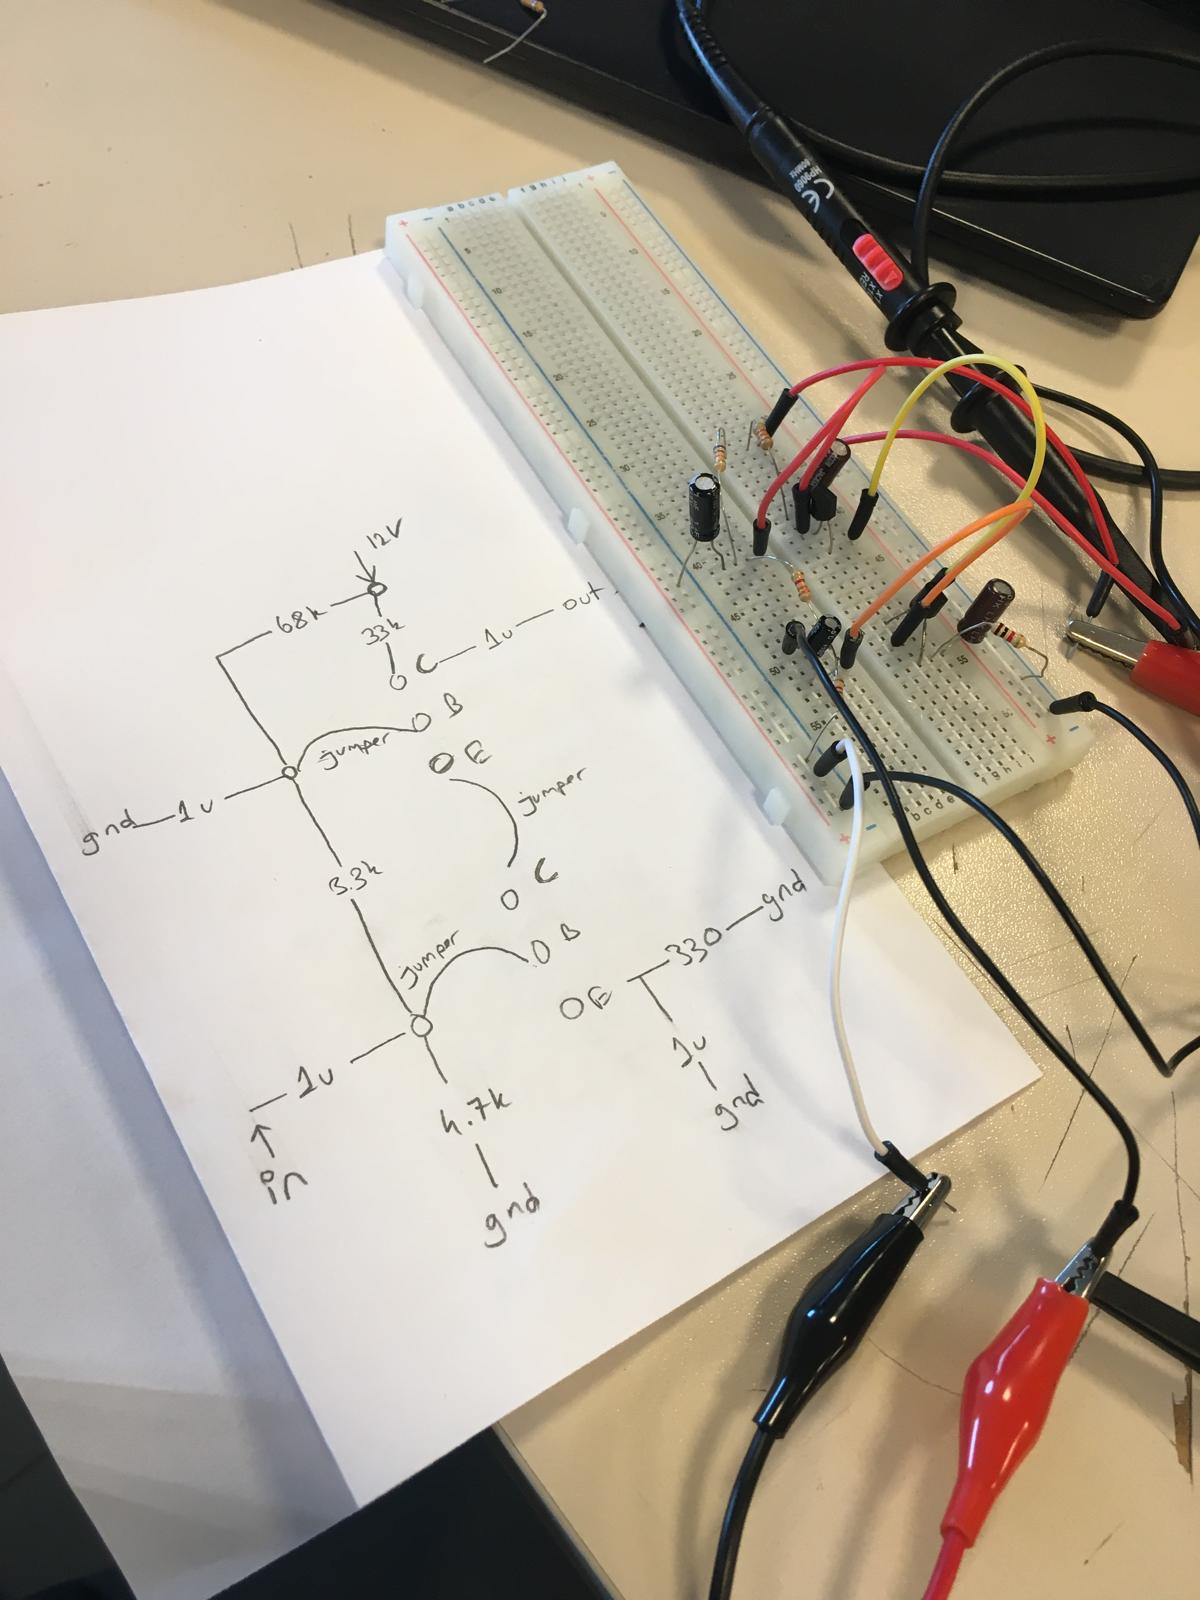
\includegraphics[width=\linewidth]{images/circuit_photo.jpeg}
        \caption{Breadboard implementation of the cascode amplifier.}
    \end{subfigure}
    \hfill
    \begin{subfigure}[t]{0.47\textwidth}
        \centering
        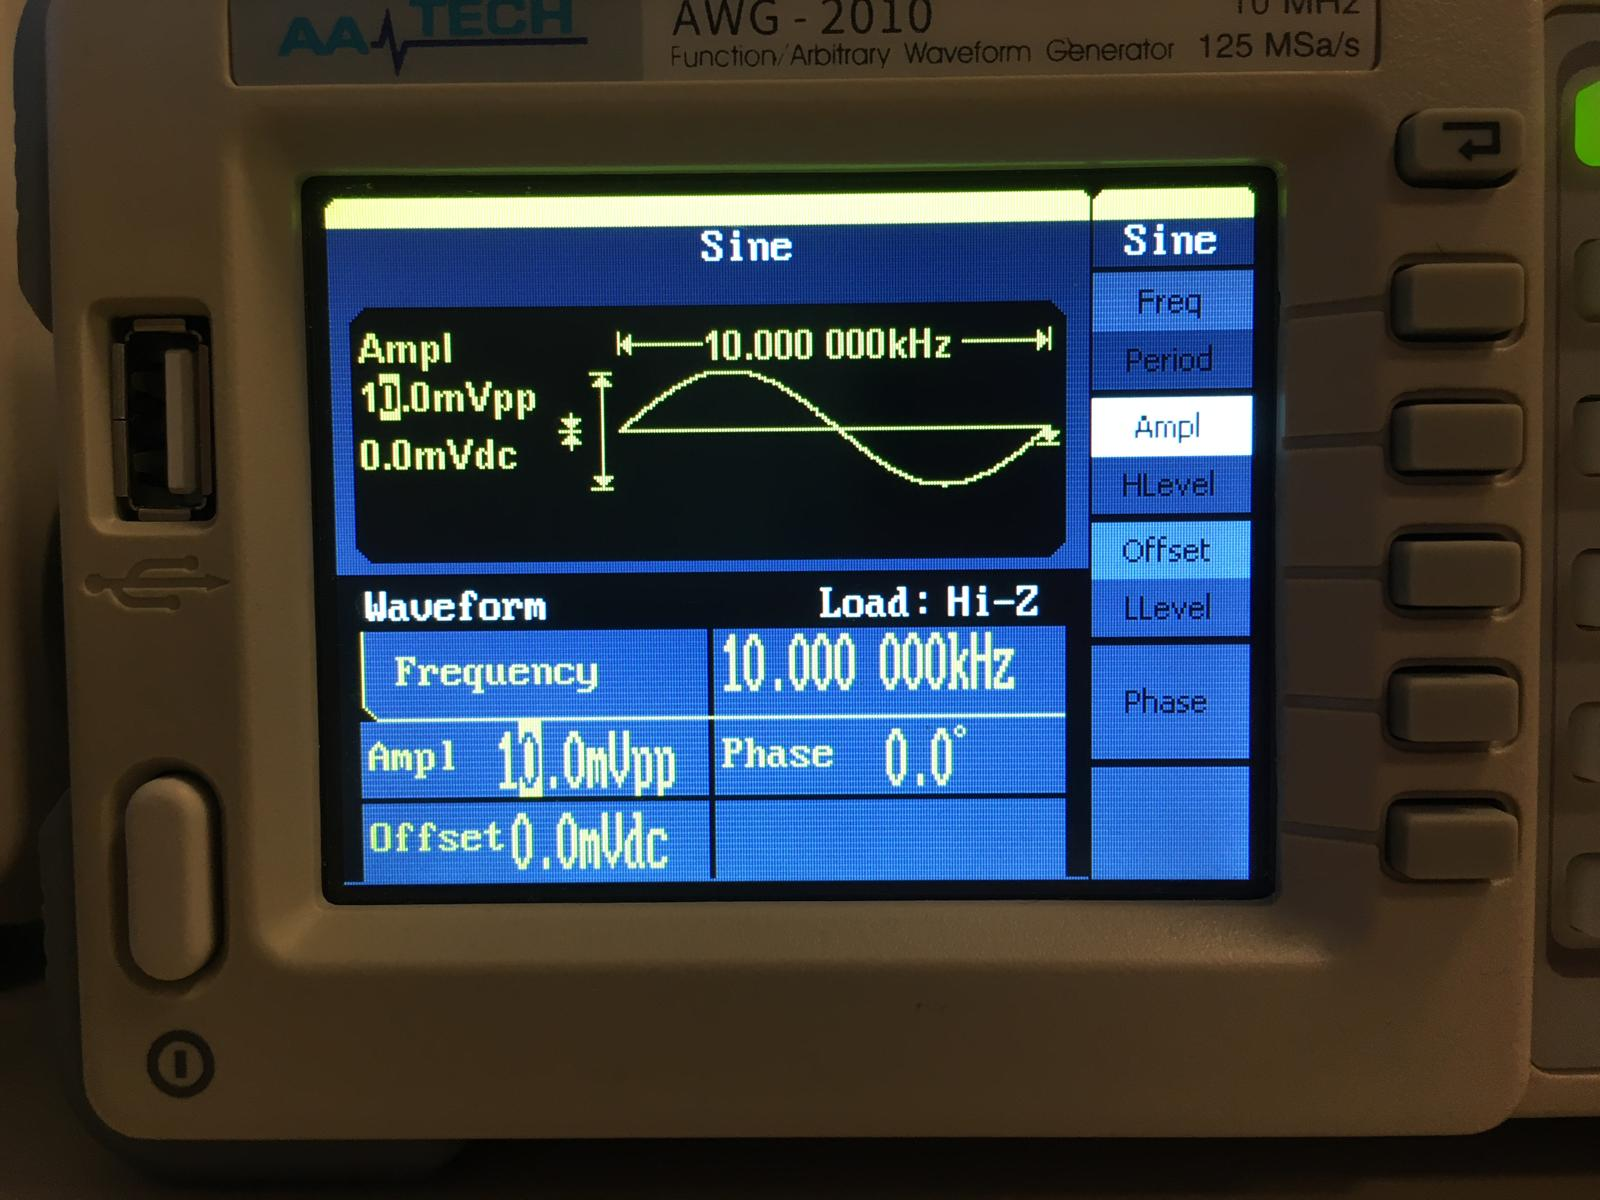
\includegraphics[width=\linewidth]{images/funcgen_photo.jpeg}
        \caption{Function generator set to 10\,mV\textsubscript{pp} at 10\,kHz.}
    \end{subfigure}
    \caption{Constructed circuit and input signal source for Task 1.}
\end{figure}

\subsubsection*{B. Initial Measurement with R4 = 330\,$\Omega$ (Clipping Observed)}

With the original R4 = 330\,$\Omega$, the function generator was set to a 10\,mV
peak-to-peak sine wave at 10\,kHz. The oscilloscope measurement showed:

\begin{itemize}
    \item Measured input ($V_{ipp}$): 31.2\,mV\textsubscript{pp} (due to noise pickup on
          the small 10\,mV signal)
    \item Measured output ($V_{opp}$): 2.6\,V\textsubscript{pp}
\end{itemize}

\noindent As seen in Figure\,\ref{fig:clipping}, the output waveform exhibited clear
\textbf{clipping}, meaning the transistor Q1 was being driven into saturation on the
negative half-cycle. This indicates that the gain with R4 = 330\,$\Omega$ was high enough
to push the output beyond the linear operating range of the amplifier.

\begin{figure}[h!]
    \centering
    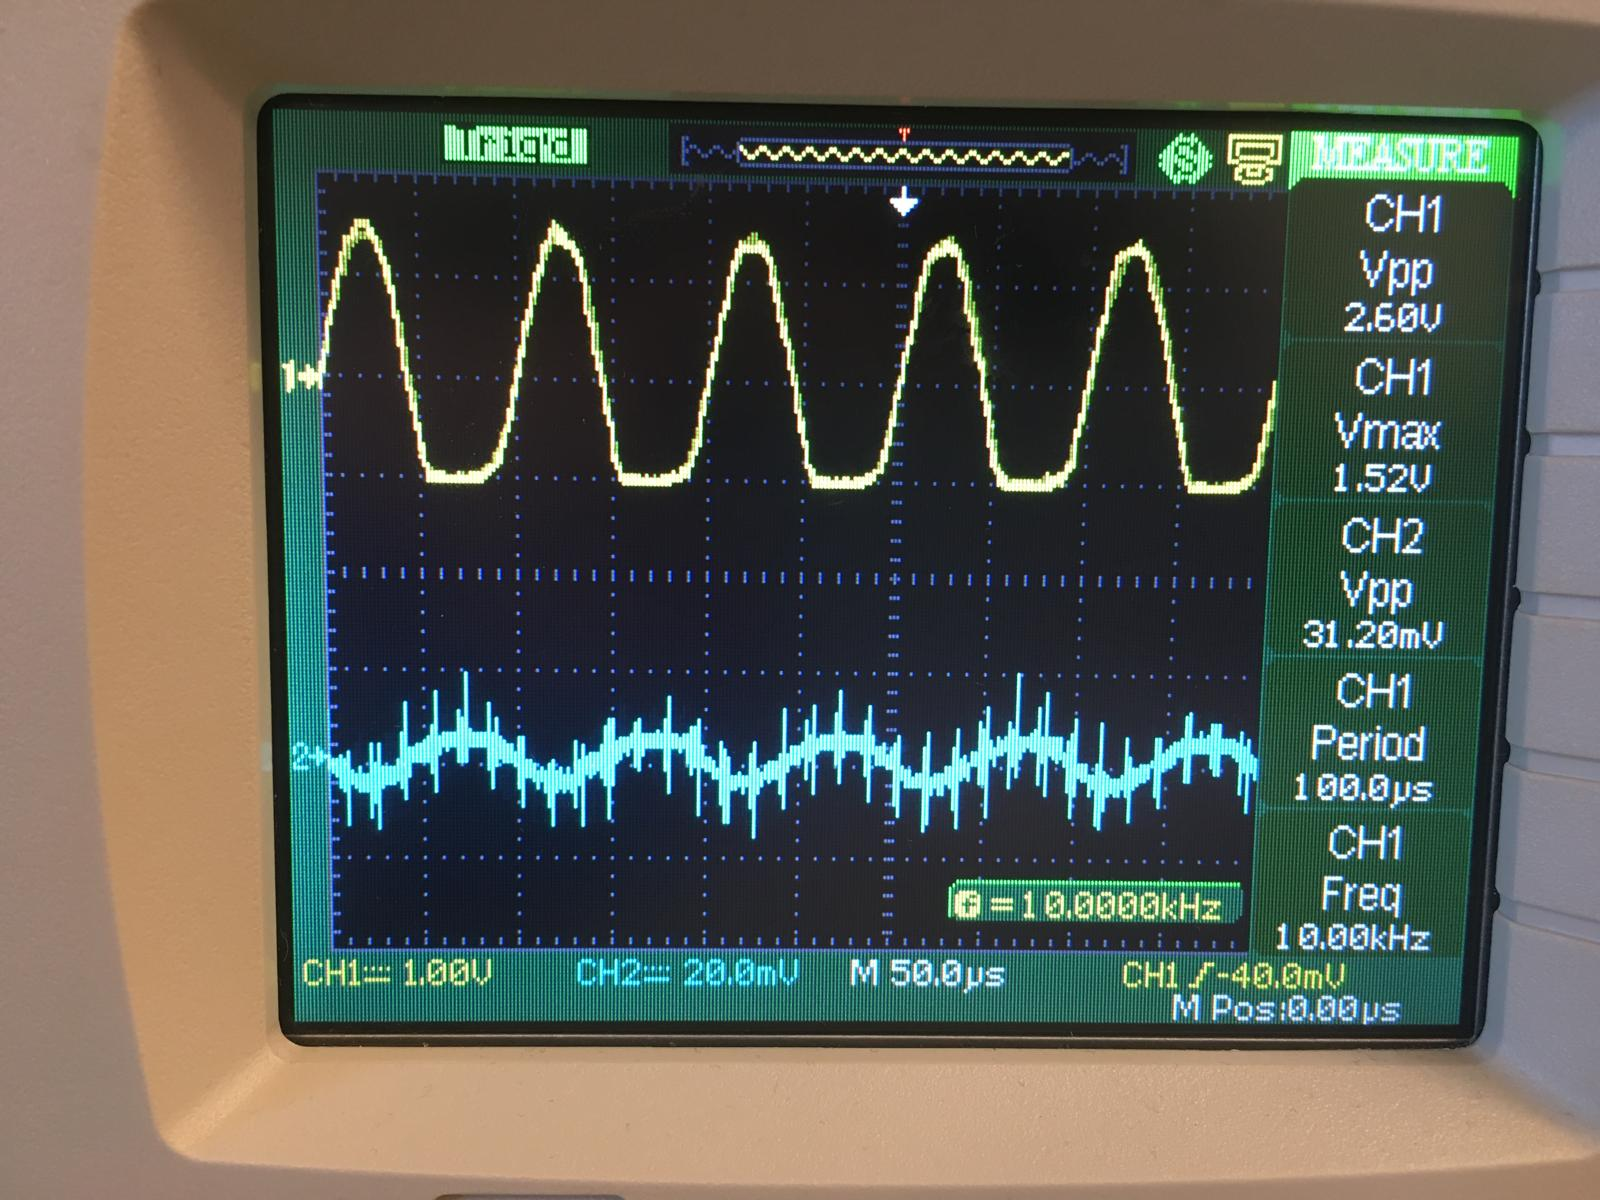
\includegraphics[width=0.65\textwidth]{images/scope_330.jpeg}
    \caption{Oscilloscope output with R4 = 330\,$\Omega$. The output waveform shows
    clipping, indicating the amplifier is operating outside its linear region.}
    \label{fig:clipping}
\end{figure}

\subsubsection*{C. Corrected Measurement with R4 = 1\,k$\Omega$}

To eliminate clipping, R4 was increased to 1\,k$\Omega$. This raises the emitter
degeneration resistance of Q2, which reduces the overall transconductance and therefore
lowers the gain, bringing the output swing back within the linear region. The measurements
with R4 = 1\,k$\Omega$ were:

\begin{itemize}
    \item Input ($V_{ipp}$): 10\,mV\textsubscript{pp} (nominal, set by function generator)
    \item Measured output ($V_{opp}$): 1.88\,V\textsubscript{pp}
\end{itemize}

\noindent The voltage gain is calculated as:

\begin{equation}
    A_v = \frac{V_{opp}}{V_{ipp}} = \frac{1.88\,\text{V}}{0.01\,\text{V}} = \mathbf{188}
\end{equation}

\noindent This is close to the target gain of 200 specified in the prelab. The small
discrepancy is attributed to component tolerances and the fact that the actual transistor
$\beta$ and $g_m$ values may differ slightly from the ideal datasheet values used in
calculations.

\begin{figure}[h!]
    \centering
    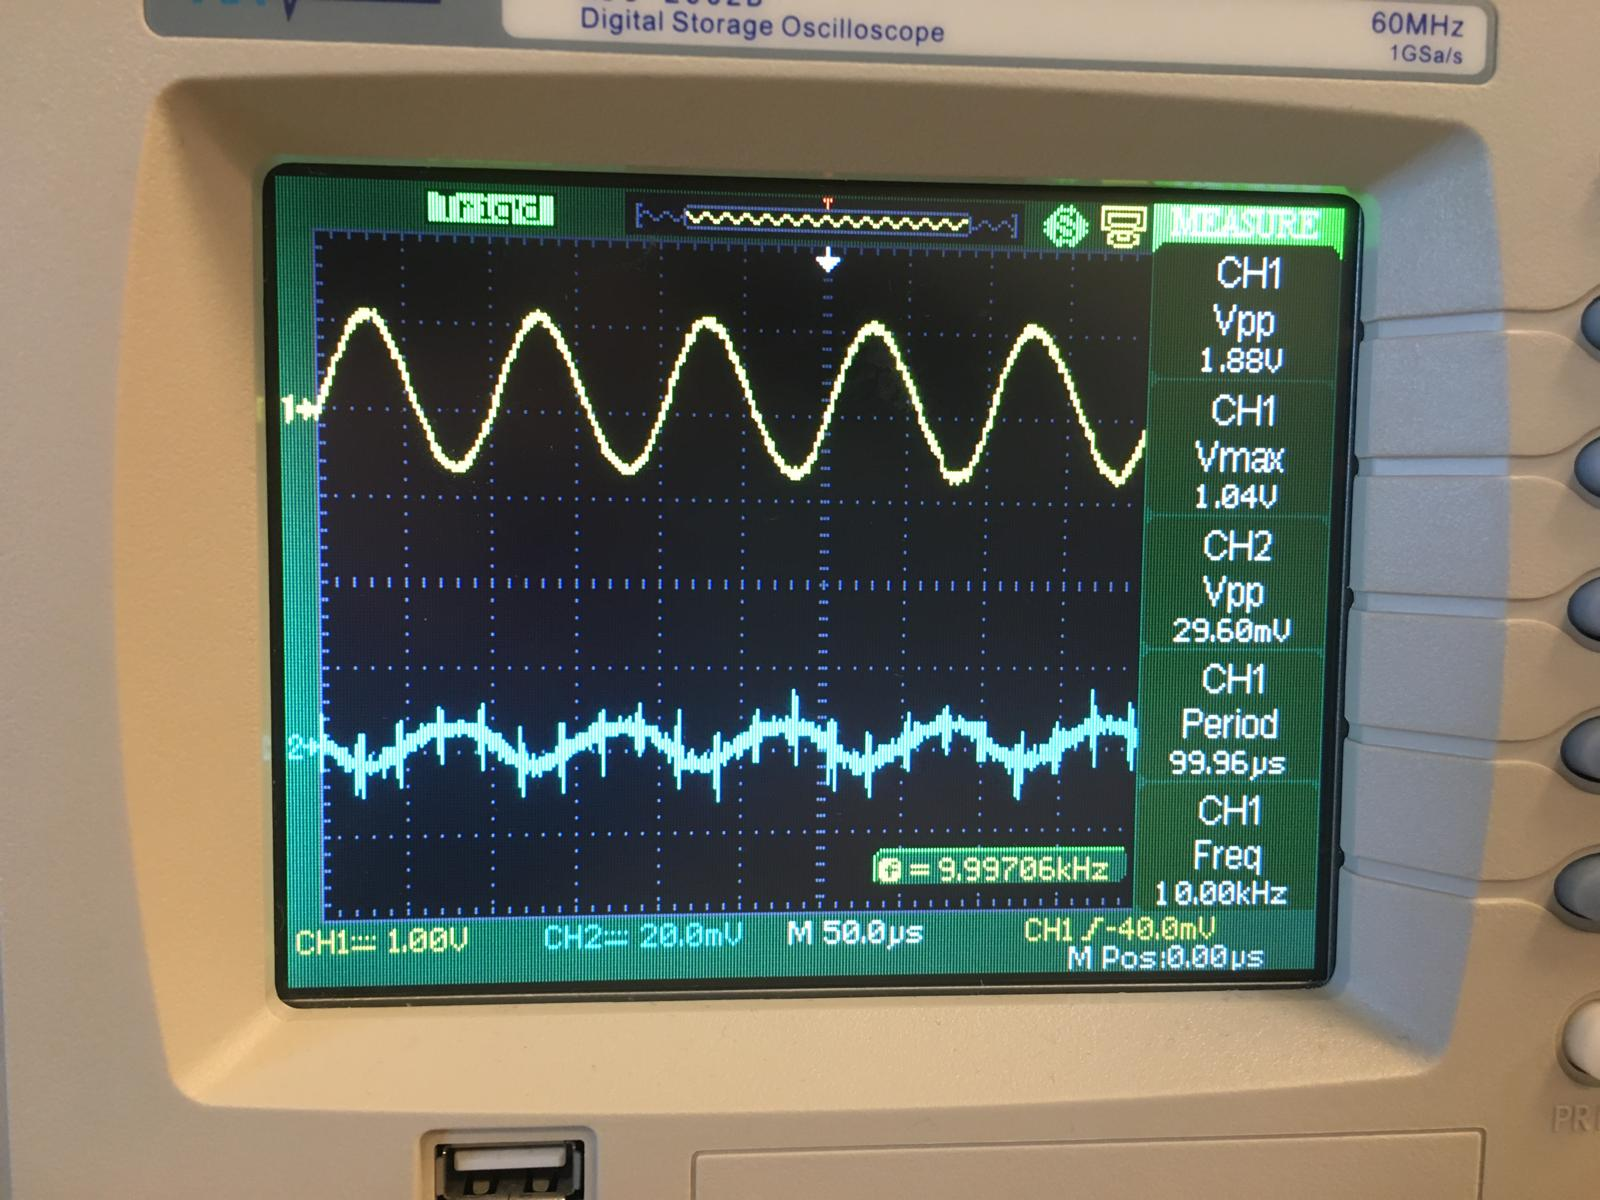
\includegraphics[width=0.65\textwidth]{images/scope_1k.jpeg}
    \caption{Oscilloscope output with R4 = 1\,k$\Omega$. The output waveform is a clean
    sinusoid with $V_{opp}$ = 1.88\,V\textsubscript{pp}, confirming linear operation and
    a gain of 188.}
    \label{fig:clean}
\end{figure}

\noindent \textbf{Comment:} The increase of R4 from 330\,$\Omega$ to 1\,k$\Omega$ resolved
the clipping by introducing stronger emitter degeneration, which trades gain for linearity.
It is also worth noting that because the input signal is only 10\,mV\textsubscript{pp},
the oscilloscope reading is susceptible to ambient noise and ground loop interference,
which explains why the scope measured 29--31\,mV rather than exactly 10\,mV at the input
node. For the gain calculation, the nominal function generator value of 10\,mV\textsubscript{pp}
is used as it represents the true input to the circuit.


\newpage

% ── TASK 2 ────────────────────────────────────
\subsection*{Task 2: Input Impedance Measurement}

\subsubsection*{A. Method}

To measure the input impedance, a potentiometer was connected in series between the 
function generator and the amplifier input, initially set to zero. The output voltage 
was monitored on the oscilloscope while the potentiometer resistance was gradually 
increased. When the output amplitude dropped to half of its original value, the 
potentiometer was removed and its resistance was measured.

This method works because the potentiometer ($R_{pot}$) and the amplifier input 
impedance ($Z_{in}$) form a voltage divider at the input:

\begin{equation}
    V_{in} = V_s \cdot \frac{Z_{in}}{Z_{in} + R_{pot}}
\end{equation}

\noindent When the output drops to half, $V_{in} = V_s / 2$, which gives:

\begin{equation}
    \frac{1}{2} = \frac{Z_{in}}{Z_{in} + R_{pot}} \implies Z_{in} = R_{pot}
\end{equation}

\noindent Therefore, the input impedance equals the potentiometer resistance at the 
half-amplitude point.

\subsubsection*{B. Results}

With the input set to 10\,mV\textsubscript{pp} at 10\,kHz, the reference output voltage 
was measured as $V_{opp} = 1.9$\,V\textsubscript{pp}. The potentiometer was increased 
until the output dropped to half:

\begin{center}
\begin{tabular}{cc}
\toprule
\textbf{Parameter} & \textbf{Value} \\
\midrule
Reference output ($V_{opp}$)       & 1.90\,V\textsubscript{pp} \\
Half-amplitude output              & 960\,mV\textsubscript{pp} \\
Potentiometer reading ($R_{pot}$)  & 2.12\,k$\Omega$ \\
\midrule
\textbf{Input Impedance} ($Z_{in}$) & \textbf{2.12\,k$\Omega$} \\
\bottomrule
\end{tabular}
\end{center}

\begin{figure}[h]
    \centering
    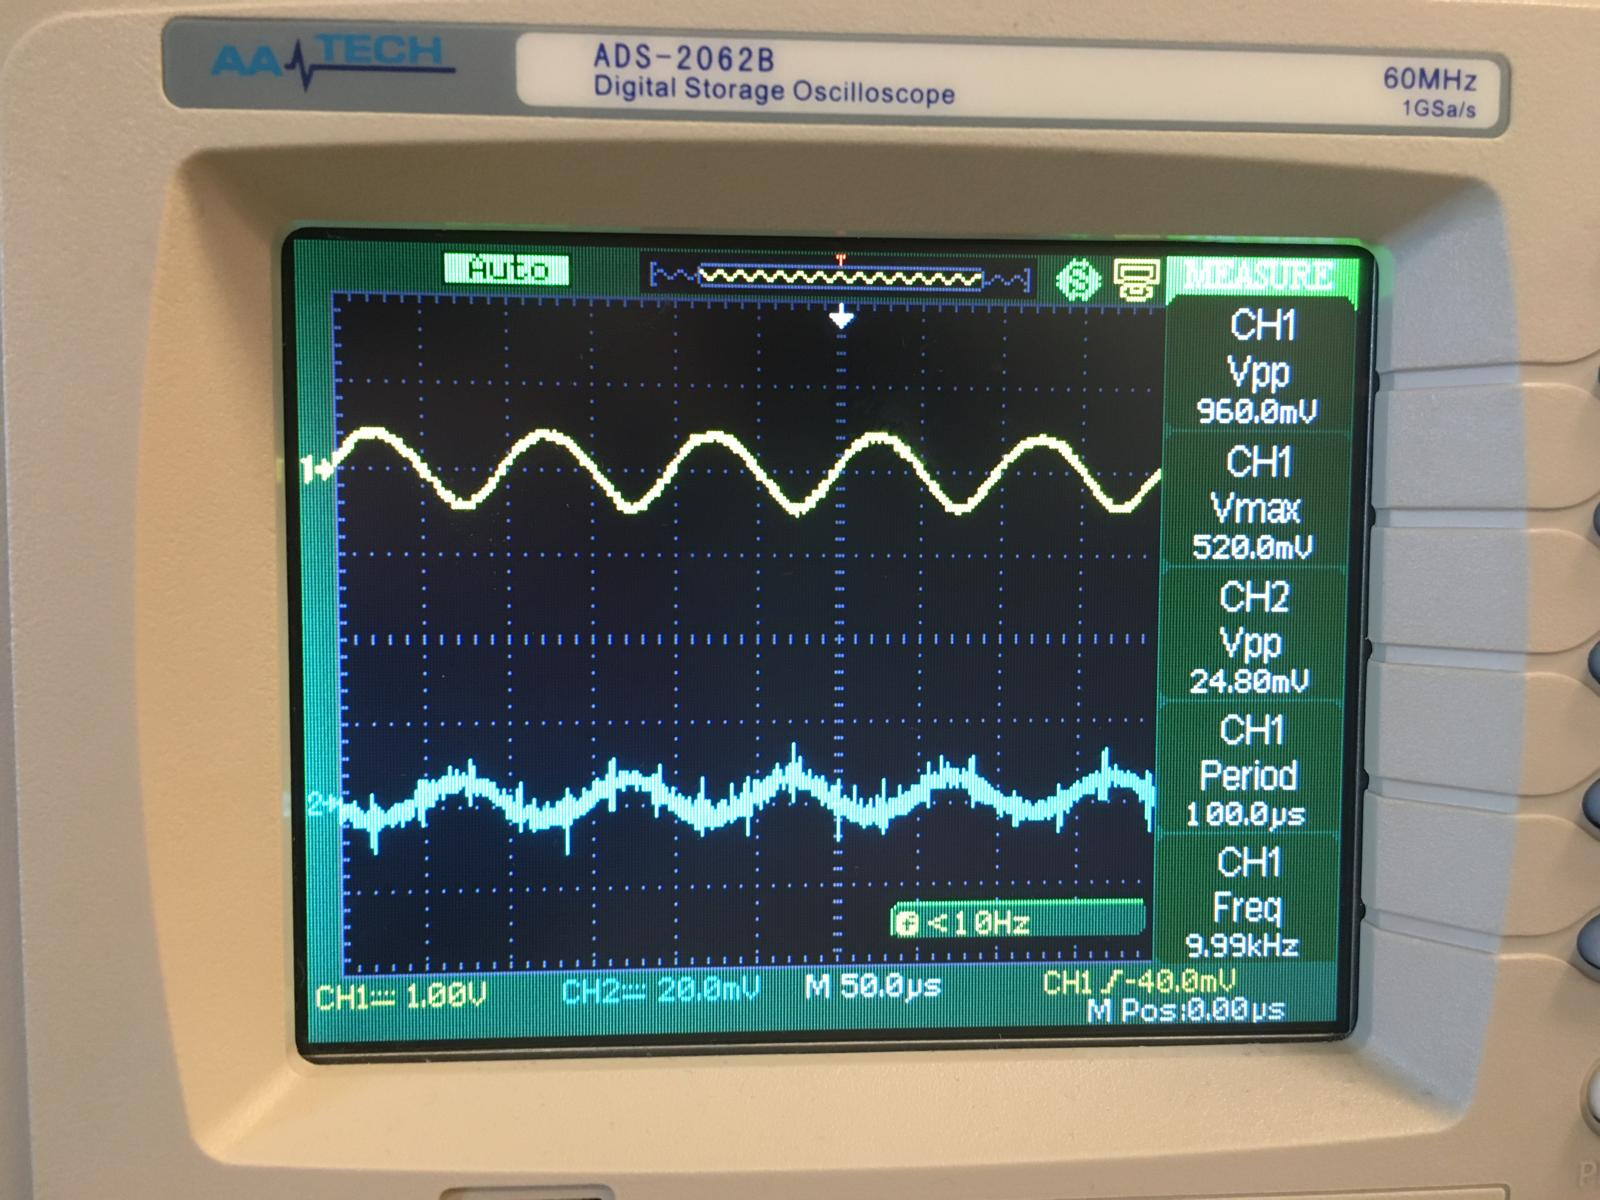
\includegraphics[width=0.50\textwidth]{images/scope_zin.jpeg}
    \caption{Oscilloscope Results}
\end{figure}

\newpage
\noindent \textbf{Comment:} The measured input impedance of 2.12\,k$\Omega$ is 
consistent with the expected value for this cascode topology. The input impedance is 
primarily determined by the parallel combination of the biasing resistors R1, R2 and 
the transistor's input resistance $r_{\pi}$, given by:

\begin{equation}
    Z_{in} = R1 \| R2 \| r_{\pi 2} \approx 68\text{k} \| 3.3\text{k} \| r_{\pi}
    \approx 2\text{--}3\,\text{k}\Omega
\end{equation}

\noindent The dominant term is R2 = 3.3\,k$\Omega$ in parallel with $r_{\pi}$, which 
pulls the input impedance down to the measured 2.12\,k$\Omega$.



% ── TASK 3 ────────────────────────────────────
\subsection*{Task 3: Output Impedance Measurement}

\subsubsection*{A. Method}

The potentiometer was removed from the input and the signal generator was reconnected
directly. The potentiometer was then connected between the output node and ground,
starting at its maximum value of 100\,k$\Omega$. Its resistance was gradually reduced
while monitoring the output on the oscilloscope. When the output dropped to half its
original amplitude, the potentiometer was removed and measured.

This works because the output impedance ($Z_{out}$) and the potentiometer ($R_{pot}$)
form a load divider at the output:

\begin{equation}
    V_{out} = V_{oc} \cdot \frac{R_{pot}}{Z_{out} + R_{pot}}
\end{equation}

\noindent At the half-amplitude point:

\begin{equation}
    \frac{1}{2} = \frac{R_{pot}}{Z_{out} + R_{pot}} \implies Z_{out} = R_{pot}
\end{equation}

\subsubsection*{B. Results}

\begin{center}
\begin{tabular}{cc}
\toprule
\textbf{Parameter} & \textbf{Value} \\
\midrule
Reference output ($V_{opp}$)        & 1.88\,V\textsubscript{pp} \\
Half-amplitude output               & 920\,mV\textsubscript{pp} \\
Potentiometer reading ($R_{pot}$)   & 24.42\,k$\Omega$ \\
\midrule
\textbf{Output Impedance} ($Z_{out}$) & \textbf{24.42\,k$\Omega$} \\
\bottomrule
\end{tabular}
\end{center}

\begin{figure}[h!]
    \centering
    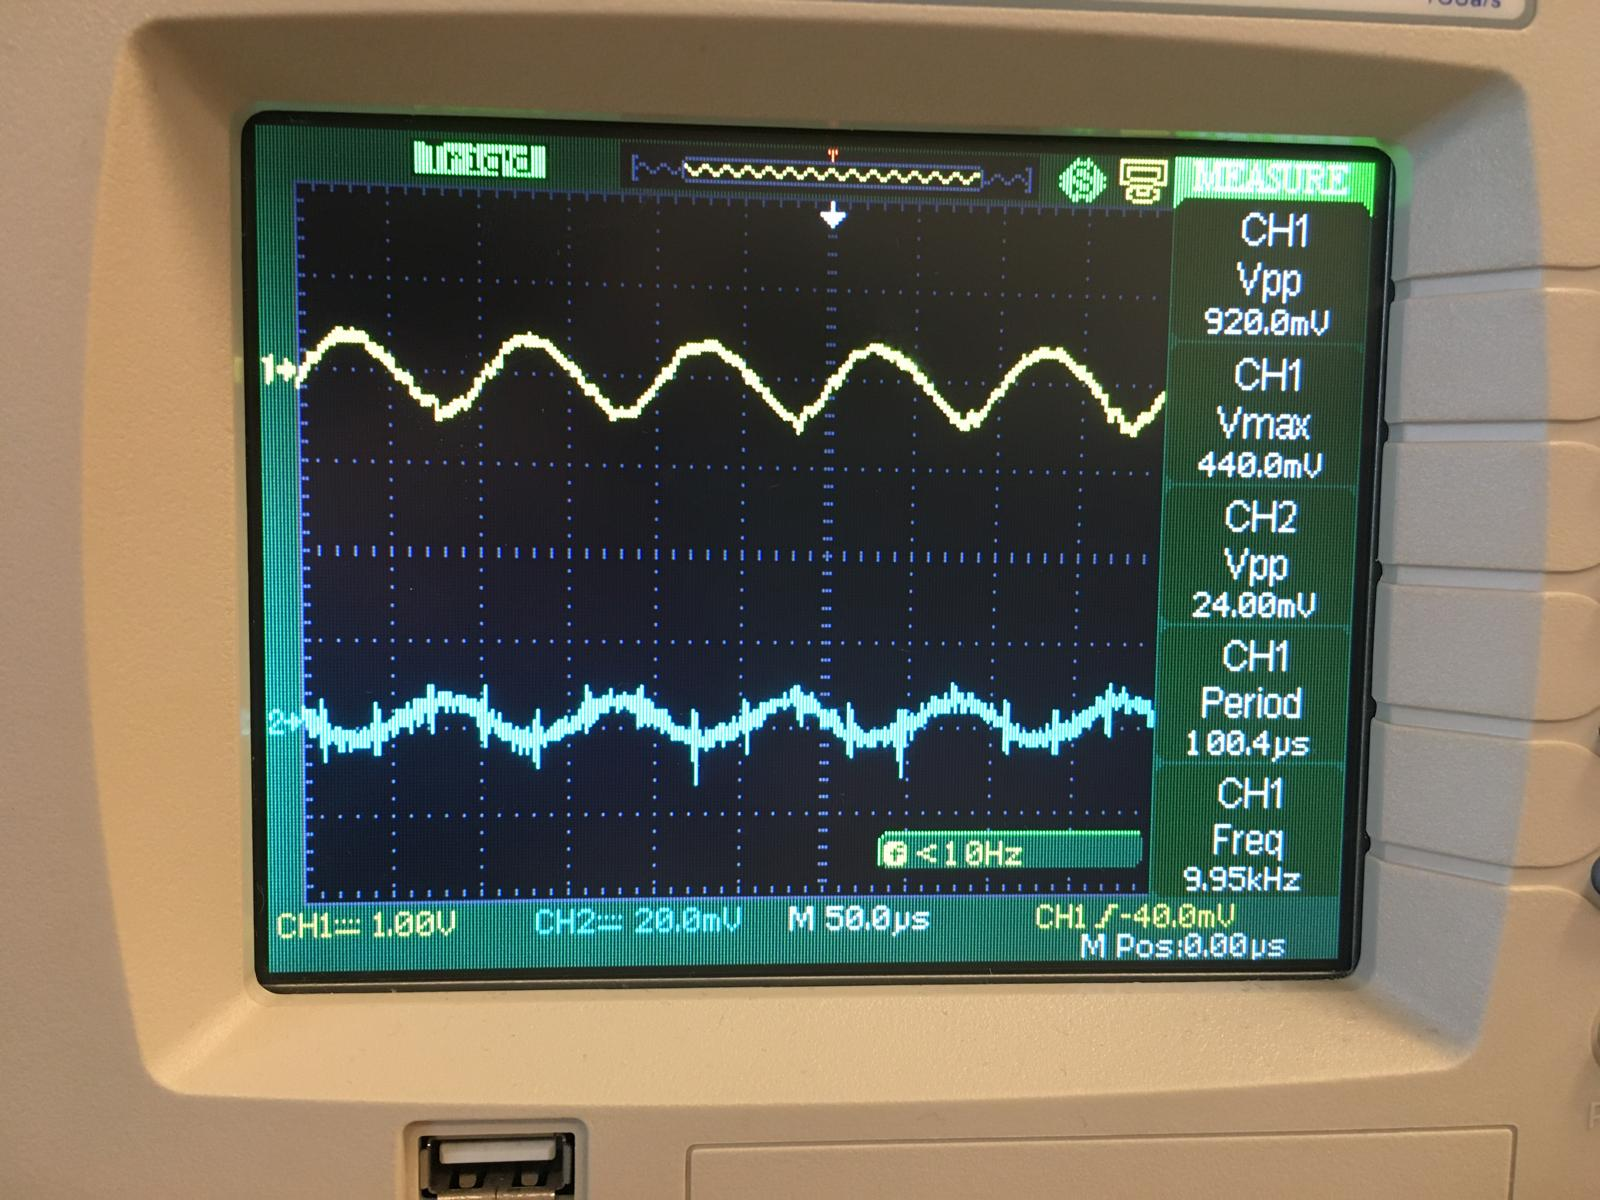
\includegraphics[width=0.60\textwidth]{images/scope_zout.jpeg}
    \caption{Output dropped to 920\,mV\textsubscript{pp} at $R_{pot}$ = 24.42\,k$\Omega$.}
\end{figure}

\noindent \textbf{Comment:} The measured output impedance of 24.42\,k$\Omega$ is 
consistent with the cascode topology, where the output impedance is approximately 
equal to R5 in parallel with the large output resistance of the cascode stage:

\begin{equation}
    Z_{out} \approx R5 \| r_{o1} \approx 33\,\text{k}\Omega \| r_{o1}
\end{equation}

\noindent Since R5 = 33\,k$\Omega$ is the dominant term, the measured 24.42\,k$\Omega$
is a reasonable result, with the difference accounted for by the finite $r_o$ of Q1
pulling the impedance slightly below R5.

% % ── TASK 4 ────────────────────────────────────



\subsection*{Task 4: NMOS Current Mirror}

\subsubsection*{A. Circuit Construction}

The NMOS current mirror (Cir.\,2.3) was constructed using two 2N7000 transistors with
the calculated R1 value. The reference current was set to 1\,mA. The current through
R\textsubscript{LOAD} was determined by measuring the voltage across it with a multimeter
and applying Ohm's law:

\begin{equation}
    I_{load} = \frac{V(R_{load})}{R_{load}}
\end{equation}

\subsubsection*{B. Results}

\begin{table}[h!]
    \centering
    \begin{tabular}{ccc}
    \toprule
    $R_{load}$ ($\Omega$) & Measured $V(R_{load})$ (V) & Calculated $I_{load}$ (mA) \\
    \midrule
    10      & 0.013  & 1.30 \\
    100     & 0.124  & 1.24 \\
    1000    & 1.275  & 1.28 \\
    10000   & 9.12   & 0.91 \\
    20000   & 11.58  & 0.58 \\
    30000   & 11.70  & 0.39 \\
    \bottomrule
    \end{tabular}
    \caption{Measured voltage and calculated current through $R_{load}$.}
\end{table}

\subsubsection*{C. Comment}

For low load resistances (10\,$\Omega$ to 1\,k$\Omega$), the current through
R\textsubscript{LOAD} remains approximately 1.2\,mA, which is close to the designed
reference current of 1\,mA. The slight excess above 1\,mA is due to component
tolerances and the finite output resistance of the MOSFET.

As R\textsubscript{LOAD} increases beyond 1\,k$\Omega$, the current drops
significantly. This occurs because a large load resistance causes the voltage at the
drain of M2 to rise:

\begin{equation}
    V_{DS2} = V_{CC} - I_{load} \cdot R_{load}
\end{equation}

\noindent When $V_{DS2}$ falls below $V_{GS} - V_{TH}$, M2 exits the saturation region
and enters the triode (linear) region, where it can no longer maintain a constant
drain current. At $R_{load}$ = 30\,k$\Omega$, the voltage across the load reaches
11.70\,V, nearly equal to $V_{CC}$ = 12\,V, confirming that M2 is fully out of
saturation and the mirror has broken down.

\noindent In summary, the current mirror operates correctly for
$R_{load} \leq 1\,\text{k}\Omega$ and fails to maintain constant current for larger
load resistances due to the MOSFET leaving saturation.



% ─────────────────────────────────────────────
%  3. CONCLUSION
% ─────────────────────────────────────────────
\section{Conclusion}

In this experiment, a BJT cascode amplifier and an NMOS current mirror were 
successfully constructed and characterised. The cascode amplifier achieved a voltage 
gain of 188, close to the target of 200, with a measured input impedance of 
2.12\,k$\Omega$ and output impedance of 24.42\,k$\Omega$. The high output impedance 
is a key advantage of the cascode topology, making it suitable for applications 
requiring high gain and high output resistance such as RF amplifiers and op-amp 
input stages.

The current mirror maintained a stable current of approximately 1.2\,mA for load 
resistances up to 1\,k$\Omega$, beyond which the current dropped as the MOSFET 
exited saturation. This highlights the importance of keeping the drain voltage of M2 
sufficiently high for correct mirror operation.

Several sources of error were observed throughout the experiment. The small 10\,mV 
input signal was susceptible to ambient noise, causing the oscilloscope to read 
slightly higher values than the actual input. Component tolerances of the resistors 
and transistor parameter variations between individual devices also contributed to 
deviations from theoretical values. Additionally, breadboard contact resistance 
introduced small but non-negligible errors, particularly at low load resistances in 
the current mirror measurements. Despite these non-idealities, the experimental 
results were in good agreement with theoretical expectations.
\end{document}
\end{document}